
\begin{figure*}[t!]
\includegraphics[width=\linewidth]{figs/KNNraw-revision.pdf}
\caption[]{End-to-End DR and k-NN runtime (top three) and returned lower dimension (bottom) over the largest UCR datasets for three different indexing routines. DROP consistently returns lower dimensional representations than conventional alternatives (FFT, PAA), and is on average faster than PAA and FFT.}
\label{fig:knnAll}
\end{figure*}

\section{Experimental Evaluation}
\label{sec:experiments}

We evaluate DROP's runtime, accuracy, and extensibility. We demonstrate that (1) DROP outperforms PAA and FFT in end-to-end workloads, (2) DROP's optimizations each contribute to performance,  and (3) DROP extends beyond time series.

\begin{comment}
\begin{enumerate}[itemsep=0.5em]
\item{DROP outperforms PAA and FFT in end-to-end, repetitive-query workloads (\S\ref{subsec:runtime}).}	
\item{DROP's optimizations for sampling, downstream task and work reuse contribute to performance (\S\ref{subsec:lesion}).}
\item{DROP's DR runtime scales with intrinsic dimensionality, independently of data size (\S\ref{subsec:scale}).}
\item{DROP extends beyond our time series case study (\S\ref{subsec:nonts}).}	
\end{enumerate}
\end{comment}

\subsection{Experimental Setup}
\label{subsec:setup}
\minihead{Implementation} We implement DROP\footnote{\href{https://github.com/stanford-futuredata/DROP}{https://github.com/stanford-futuredata/DROP}} in Java using \red{the multi-threaded Matrix-Toolkits-Java (MTJ) library~\cite{mtj}, and netlib-java~\cite{netlib} linked against Intel MKL~\cite{mkl} for compute-intensive linear algebra operations. 
We use multi-threaded JTransforms~\cite{jtransforms} for FFT, and implement multi-threaded PAA from scratch.}
%To provide an apples-to-apples comparison with our single-core PAA implementation, we disable multithreading in MTJ---enabling multi-core will equally improve all PCA-based methods across the board, including DROP, relative to PAA.
We use \red{the} Statistical Machine Intelligence and Learning Engine (SMILE) library~\cite{smile} for k-NN {and k-means}. 

\begin{comment}
\minihead{Environment} We use a server with \red{two Intel Xeon E5-2690v4 @ 2.60Ghz CPUs, each with 14 physical and 28 virtual cores (with hyper-threading). The server contains 512GB of RAM.}
We exclude data loading and parsing time.
\end{comment}

\minihead{Datasets} 
%To showcase DROP's performance in an end-to-end setting and contributions from each optimization, we use several real world datasets.
We first consider the UCR Time Series Classification Archive~\cite{ucr}, excluding datasets with fewer than 1 million entries, and fewer datapoints than dimensionality, leaving 14 datasets. 
%We also consider a larger, labeled earthquake dataset from XXX~\cite{quake}.
As these are all relatively small time series, we consider four additional datasets to showcase DROP's scalability and generalizability: the MNIST digits dataset~\cite{mnist}, the FMA featurized music dataset~\cite{fma}, a sentiment analysis IMDb dataset~\cite{imdb}, and the fashion MNIST dataset~\cite{fashion}. 

\minihead{DROP Configuration} We use a runtime model for k-NN and k-means computed via polynomial interpolation on data of varying dimension.
While the model is an optional input parameter, any function estimation routine can estimate it given black-box access to the downstream workload.
To evaluate sensitivity to runtime model, we report on the effect of operating without it (i.e., sample until convergence).
We set $TLB$ constraints such that k-NN accuracy remains unchanged, corresponding to $B = 0.99$  for the UCR data.
We use a default sampling schedule that begins with and increases by $1\%$ of the input.
It is possible to optimize (and perhaps overfit) this schedule in future work (\S\ref{subsec:disc}), but we provide a conservative, general schedule as a proof of concept.
%%%%We further discuss sampling schedules and properties that make a dataset amenable to DROP in \S\ref{subsec:disc}. 


\minihead{Baselines} We report runtime, accuracy, and dimensionality compared to FFT, PAA, PCA via SVD-Halko, and PCA via SVD. 
Each computes a transformation over all the data, then performs binary search to identify the lowest dimensionality that satisfies the target $TLB$. 
%%%%We further discuss choice of PCA subroutine in \S\ref{subsec:pcaexp}. 

\minihead{Similarity Search/k-NN Setup} 
We primarily consider k-NN in our evaluation as in~\cite{keogh-study}, but also briefly validate k-means performance.
%\red{Further, adopting k-NN (and, k-means in \S\ref{subsec:nonts}), which is not a classically supported relational operator, as our target task demonstrates that simple runtime estimation routines can be extended to time-series-specific  operators.}
To evaluate DR performance when used with downstream indexes, we vary k-NN's multidimensional index structure: cover trees~\cite{ctree}, K-D trees~\cite{kdtree}, or no index. 

End-to-end performance depends on the number of queries in the workload, and DROP is optimized for the repeated-query use case. 
Due to the small size of the UCR datasets, we choose a 1:50 ratio of data indexed to number of query points, and vary this index-query ratio in later microbenchmarks and experiments. 
We also provide a cost model for assessing the break-even point that balances the cost of a given DR technique against its indexing benefits.

%%%IT WAS HERE BEFORE


\subsection{DROP Performance}
\label{subsec:runtime}


We evaluate DROP's performance compared to PAA and FFT using the time series case study extended from~\cite{keogh-study}. 

\minihead{k-NN Performance} We summarize DROP's results on a 1-Nearest Neighbor classification in Figure~\ref{fig:knnAll}.
We display the end-to-end runtime of DROP, PAA, and FFT for each of the considered index structures: no index, K-D trees, cover trees. 
We display the size of the returned dimension for the no indexing scenario, as the other two scenarios return near \red{identical values.
This occurs as many of the datasets used in this experiment are small and possess low intrinsic dimensionality that DROP quickly identifies
}
We do not display k-NN accuracy as all techniques meet the $TLB$ constraint, and achieve the same accuracy within $1\%$.

On average, DROP returns transformations that are $2.3\times$ and  $1.4\times$ smaller than PAA and FFT, translating to significantly smaller k-NN query time. 
End-to-end runtime with DROP is on average \red{$2.2\times$ and $1.4\times$ (up to $10\times$ and $3.9\times$)} faster than PAA and FFT, respectively, when using brute force linear search,  \red{$2.3\times$ and $1.2\times$ (up to $16\times$ and $3.6\times$)}  faster when using K-D trees, and \red{$1.9\times$ and $1.2\times$ (up to $5.8\times$ and $2.6\times$)} faster when using cover trees.
When evaluating Figure~\ref{fig:knnAll}, it becomes clear that DROP's runtime improvement is data dependent for both smaller datasets, and for datasets that do not possess a low intrinsic dimension (such as Phoneme, elaborated on in \S\ref{subsec:lesion})
Determining if DROP is a good fit for a dataset is an exciting area for future work (\S\ref{subsec:disc}).

%We demonstrate in our lesion study in \S\ref{subsec:lesion} that DROP also outperforms our baseline PCA via SVD implementation, as well as our SVD-Halko implementation. 

%When evaluating Figure~\ref{fig:knnAll}, it becomes clear that DROP's runtime improvement is data dependent for both smaller datasets, and for datasets that do not possess a low intrinsic dimension (such as Phoneme, elaborated on in \S\ref{subsec:lesion}). 
%Thus, in the end of the evaluation section, we provide guidelines on how to determine if DROP is a good fit for a dataset. 

\minihead{Varying Index-Query Ratio} DROP is optimized for a low index-query ratio, as in many streaming and/or high-volume data use cases.
If there are many more data points queried than used for constructing an index, but not enough such that expensive, na\"ive PCA is justified, DROP will outperform alternatives. 
A natural question that arises is: at what scale is it beneficial to use DROP?
While domain experts are typically aware of the scale of their workloads, we provide a heuristic to answer this question given rough runtime and cardinality estimates of the downstream task and the alternative DR technique in consideration.

Let $x_d$ and $x_a$ be the per-query runtime of running a downstream task with the output of DROP and a given alternative method, respectively. 
Let $r_d$ and $r_a$ denote the amortized per-datapoint runtime of DROP and the alternative method, respectively. 
Let $n_i$ and $n_q$ the number of indexed and queried points. 
DROP is faster when $n_q x_d + n_i r_d < n_q x_a + n_i r_a$.

To verify, we obtained estimates of the above and empirically validate when running k-NN using cover trees (Figure~\ref{fig:query}).
We first found that in the 1:1 index-query ratio setting, DROP should be slower than PAA and FFT, as observed. 
However, as we decrease the ratio, DROP becomes faster, with a break-even point of slightly lower than 1:3. 
We show that DROP does indeed outperform PAA \red{and FFT} in the 1:5 index-query ratio case, where it is is on average \red{$1.51\times$} faster than PAA and \red{$1.03\times$} faster than FFT. 
As the ratio decreases to 1:50, DROP is up to \red{$1.9\times$} faster than alternatives.  


\begin{figure}
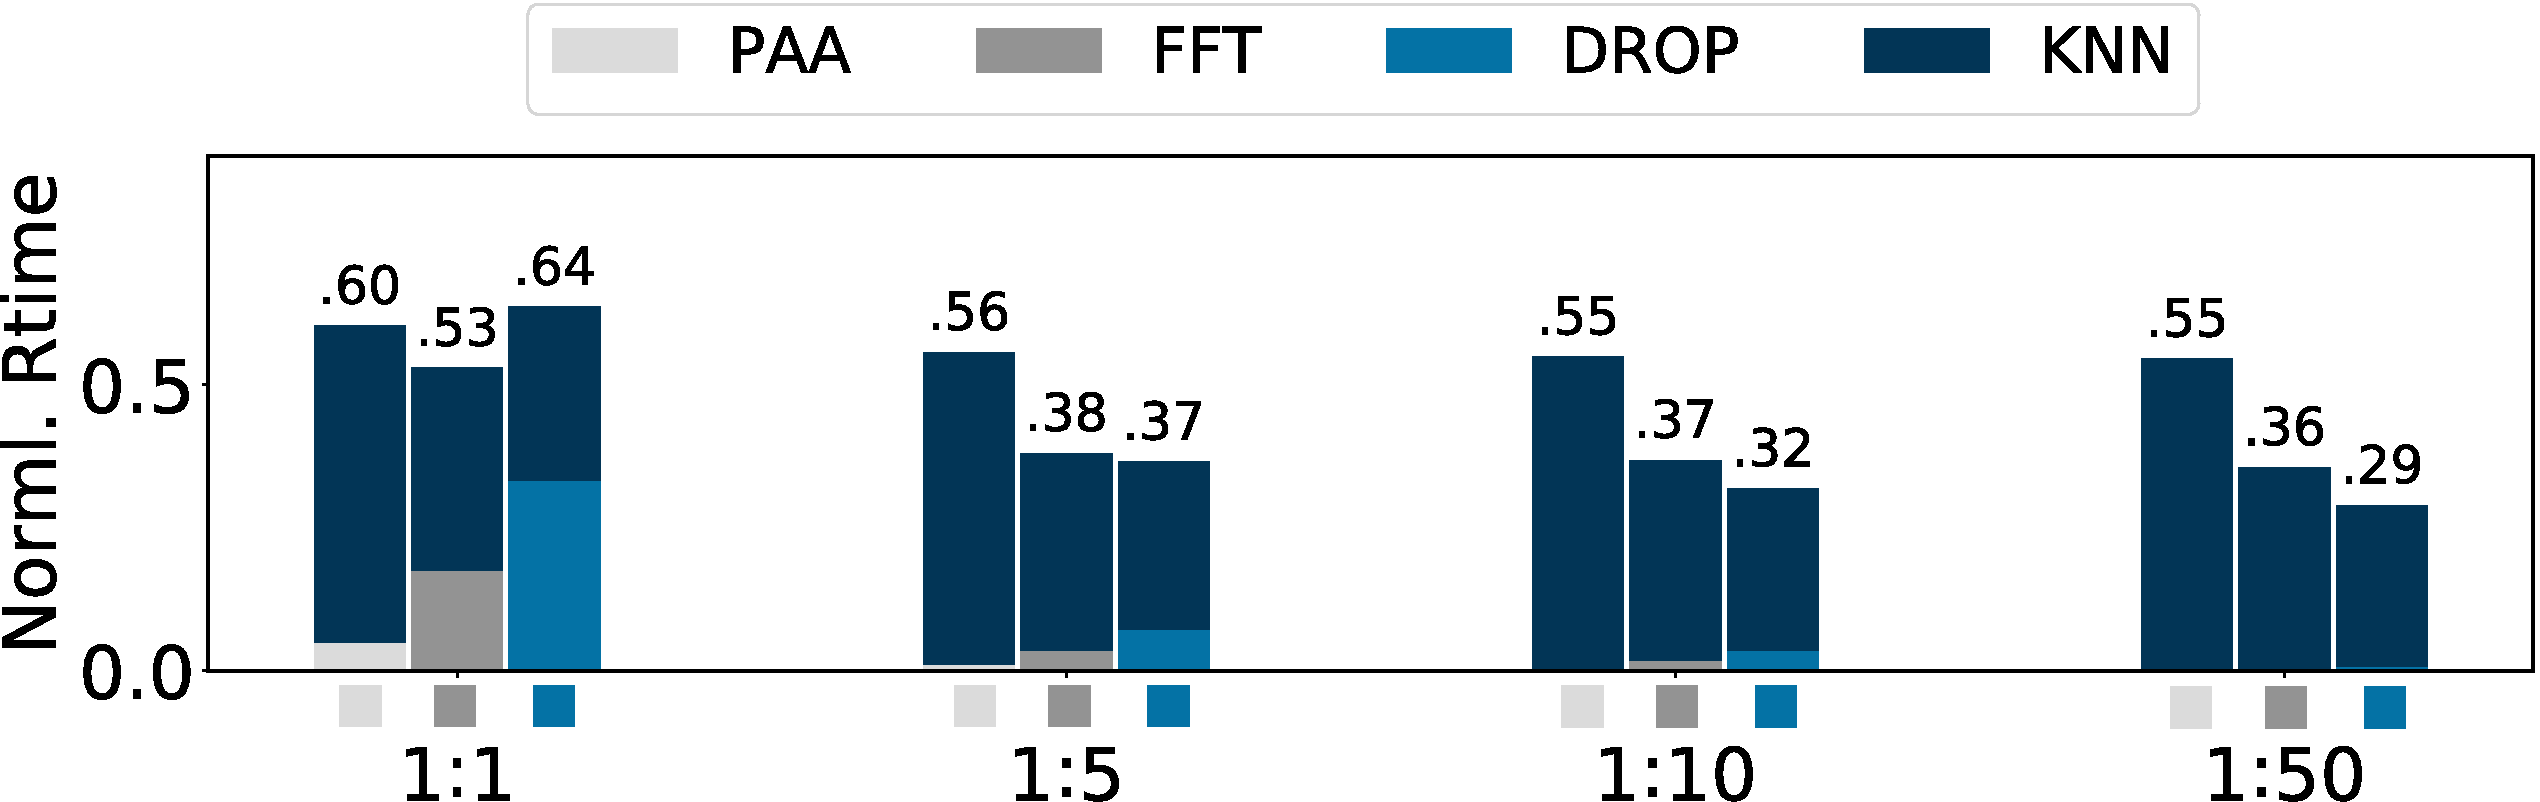
\includegraphics[width=\linewidth]{figs/query-rev.pdf}
\caption[]{Effect of decreasing the index-query ratio. As an index is queried more frequently, DROP's relative runtime benefit  increases.}
\label{fig:query}
\end{figure}

\red{
\minihead{Time Series Similarity Search Extensions}
Given the breadth of research in time series indexing, we evaluate how DROP, a general operator for PCA, compares to time series indexes. 
As a preliminary evaluation, we consider iSAX2+~\cite{isax}, a state-of-the-art indexing tool, in a 1:1 index-query ratio setting, using a publicly available Java implementation~\cite{isaxcode}. 
While these indexing techniques also optimize for the low index-query ratio setting, we find index construction to be a large bottleneck in these workloads. 
For iSax2+, index construction is on average $143\times$ (up to $389\times$) slower than DR via DROP, but is on average only $11.3\times$ faster than k-NN on the reduced space.  However, given high enough query workload, these specialized techniques will surpass DROP.


We also verify that DROP is able to perform well when using downstream similarity search tasks relying on alternative distance metrics, namely, Dynamic Time Warping (DTW)---a commonly used distance measure in the literature~\cite{isaxorig}. 
As proof-of-concept, we implement a 1-NN task using DTW with a 1:1 index-query ratio, and find that even with this high ratio, DROP provides on average $1.2\times$ and $1.3\times$ runtime improvement over PAA and FFT, respectively.
%As DTW is known to be incredibly slow~\cite{dtwslow}, it is unsurprising that DROP provides large runtime benefits for tasks using DTW without additional pruning---in terms of absolute runtime, DROP saves 2.8 minutes on the FordA dataset compared to PAA, and 2.2 minutes on the wafer dataset compared to FFT.

%Finally, as the considered time series are fairly short, we perform the same experiment over a standard gaussian random walk synthetic dataset~\cite{coconut,ssh} consisting of 50,000 time series of dimension 10,000. 
%Each time series is generated by, for each time step, generating a random value distributed via standard normal distribution, and adding it to the running sum of all previous time steps. 
%We find that DROP takes 4150ms to complete, whereas PAA and FFT take 5523ms (1.3$\times$ faster) and 15329ms (3.7$\times$ faster), respectively. 
}


\subsection{Factor Analysis}
\label{subsec:lesion}


We perform a factor analysis of the incremental runtime contributions of each of DROP's components compared to baseline SVD methods. 
We only display the results of k-NN with cover trees; the results hold for the other indexes.
We use a 1:1 index-query ratio \red{with data inflated by 5$\times$} to better highlight the effects of each contribution to the DR routine.%, and display average results over the UCR datasets in Figure~\ref{fig:lesion}, excluding Phoneme.


\begin{figure}
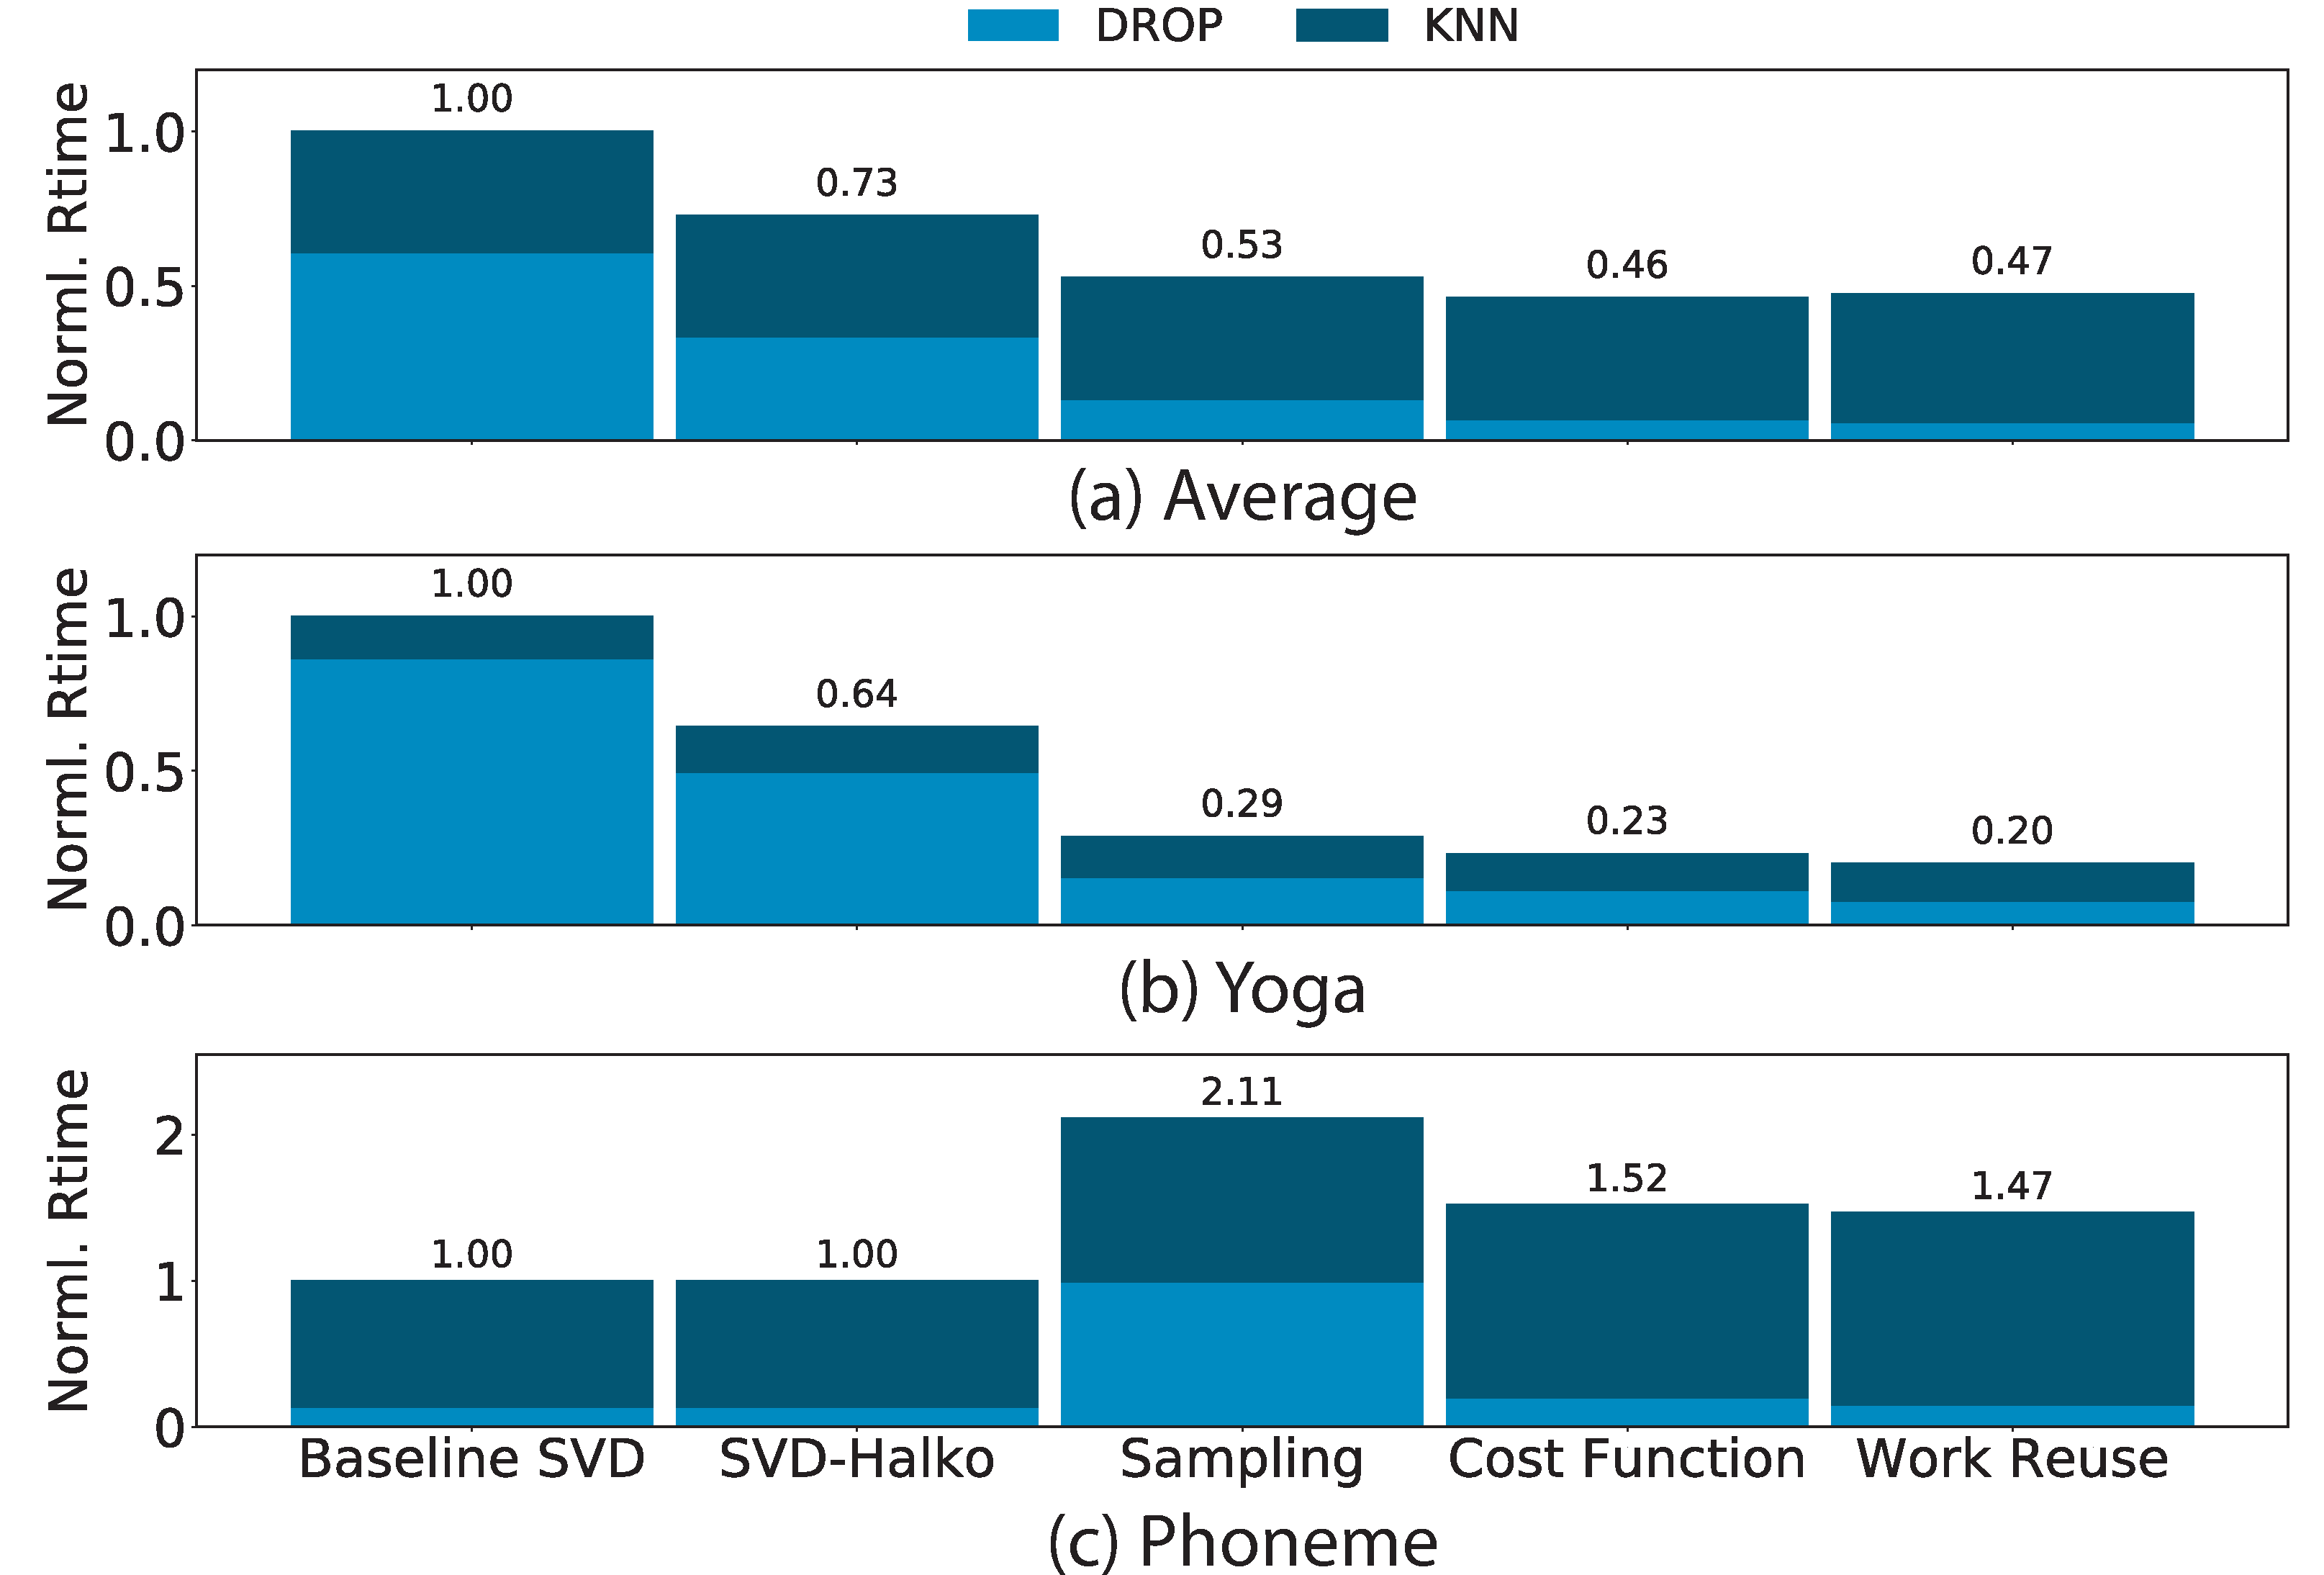
\includegraphics[width=\linewidth]{figs/lesion-all.pdf}
\caption[]{Factor Analysis demonstrating average optimization improvement (a), and sample datasets that are amenable to (b) and operate poorly (c) with DROP}
\label{fig:lesion}
\end{figure}

Figure~\ref{fig:lesion} first demonstrates the boost from using SVD-Halko over a na\"ive implementation of PCA via SVD, which comes from not computing the full transformation a priori, incrementally binary searching as needed. 
It then shows the runtime boost obtained from running on samples until convergence, where DROP samples and terminates after the returned lower dimension from each iteration plateaus.
This represents the na\"ive sampling-until-convergence approach that DROP defaults to sans user-specified cost model.
We finally introduce cost based optimization and work reuse.
Each of these optimizations improves runtime, with the exception of work reuse, which has a negligible impact on average but disproportionately impacts certain datasets. 

\begin{comment}
\red{On average, DROP is $2.1\times$ faster (up to $41\times$) than PCA via SVD, and $1.6\times$ faster than SVD-Halko (up to $3.3\times$). DROP with cost-based optimization is faster than  sampling to convergence by $1.2\times$ on average, but this default strategy is still $1.4\times$ faster than SVD-Halko on average.}


\begin{comment}
\begin{figure}
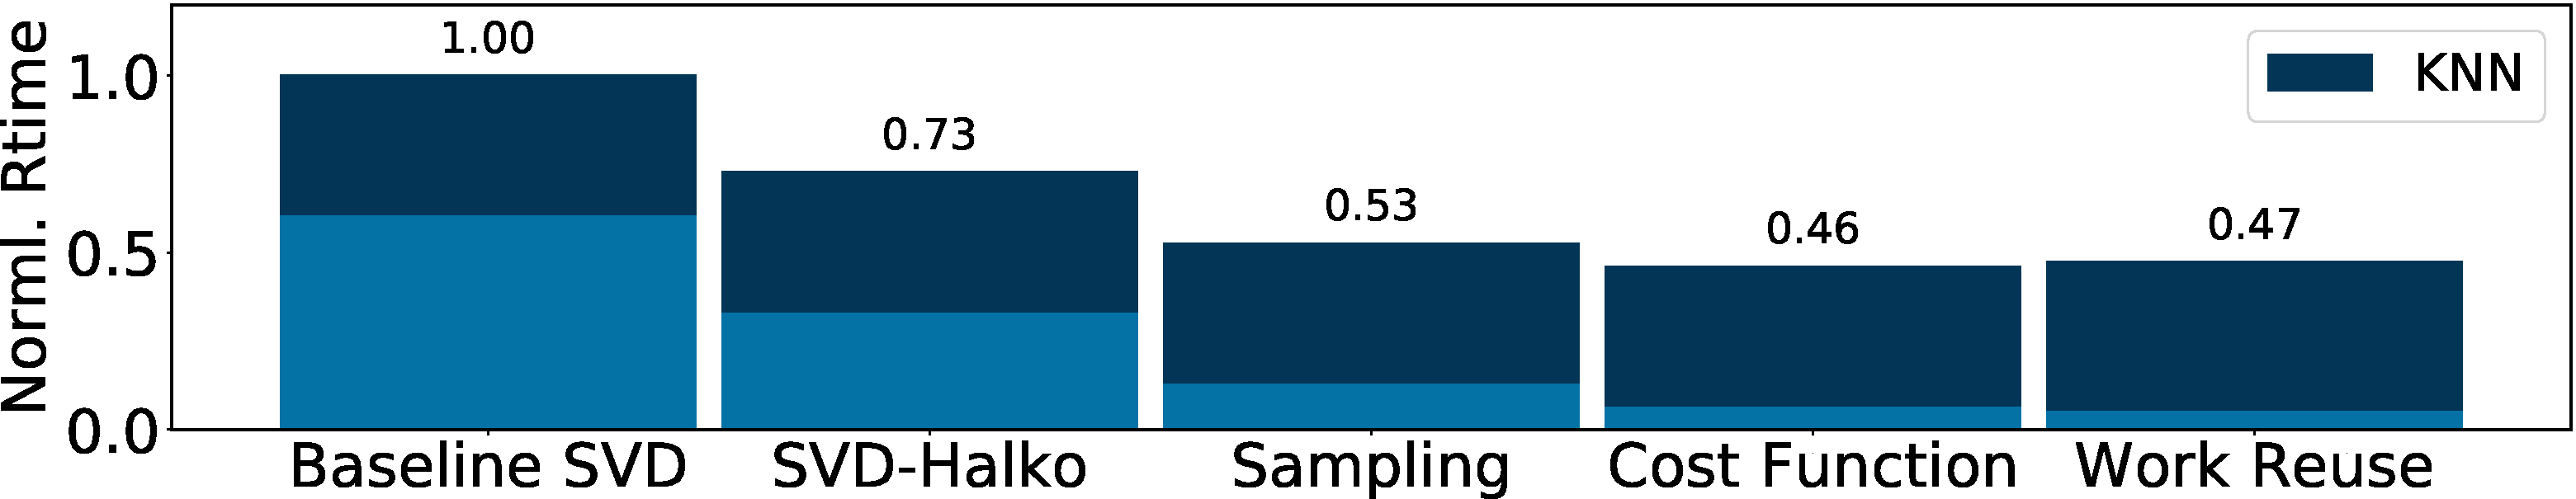
\includegraphics[width=\linewidth]{figs/lesion-rev.pdf}
\caption[]{Average result of lesion study over the UCR datasets.}
\label{fig:lesion}
\end{figure}

\begin{figure}
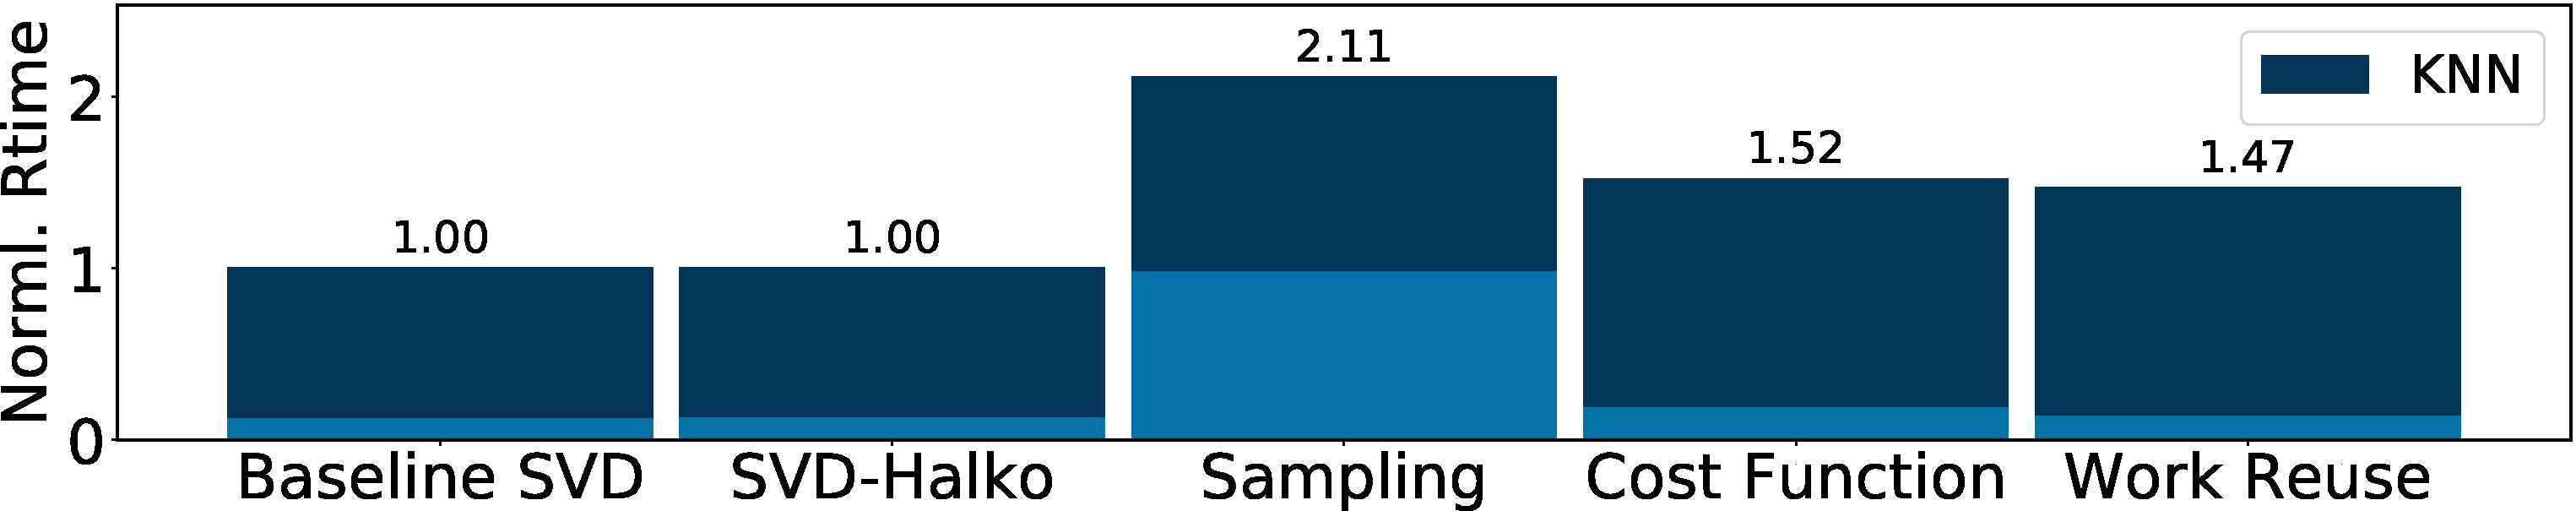
\includegraphics[width=\linewidth]{figs/phoneme-rev.pdf}
\caption[]{Lesion study of the UCR phoneme, a dataset with high intrinsic dimensionality, meaning sampling to convergence is orders of magnitude slower than a batch SVD. DROP's cost function enables it to terminate in advance, returning a higher dimensional basis to minimize reduce overall compute.}
\label{fig:phoneme_lesion}
\end{figure}

\begin{figure}
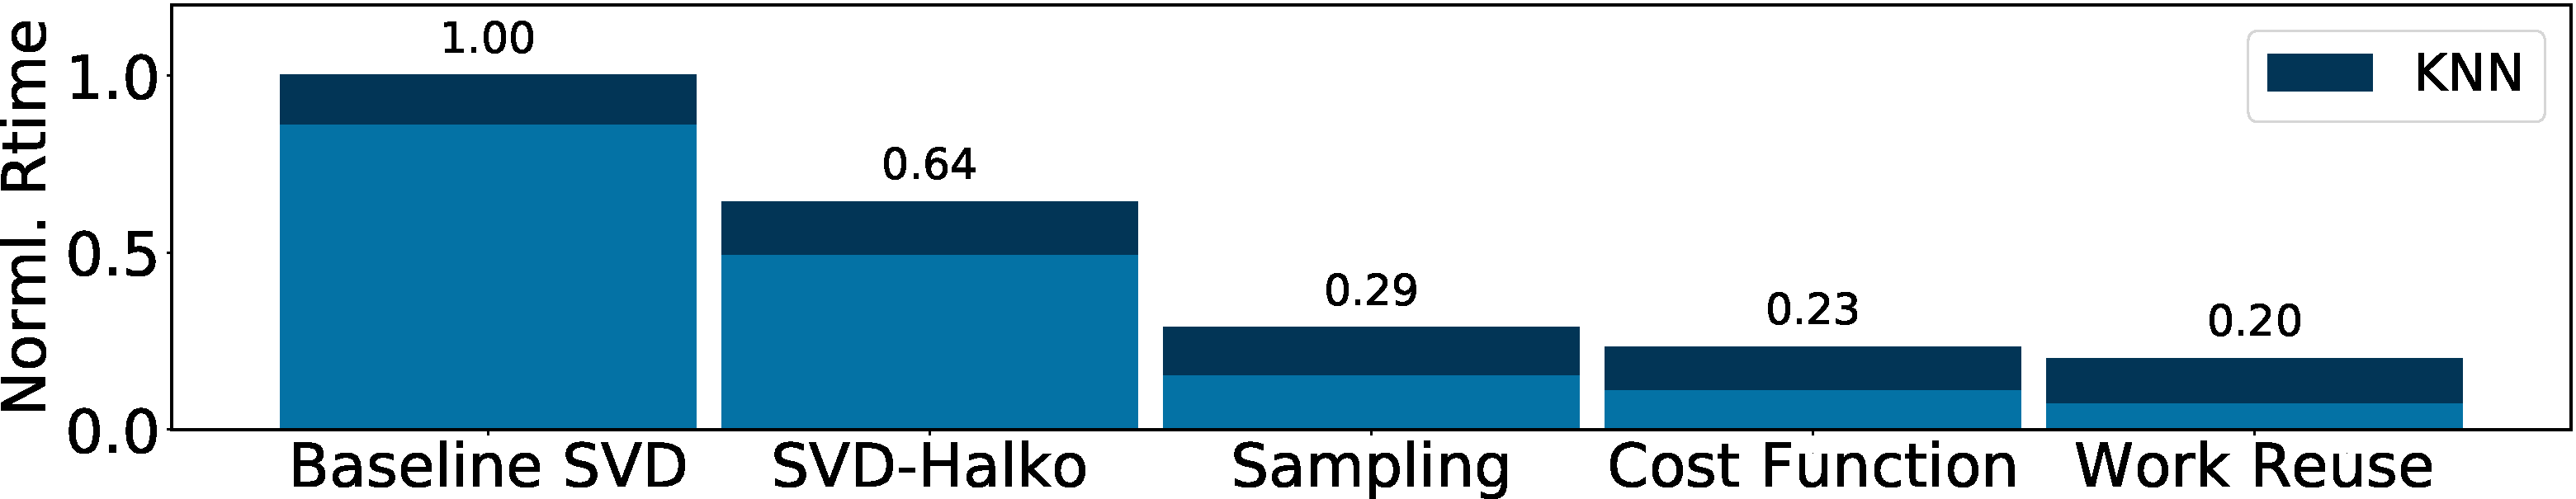
\includegraphics[width=\linewidth]{figs/yoga-rev.pdf}
\caption[]{Lesion study over the UCR yoga dataset. Work reuse provides a $15\%$ runtime improvement.}
\label{fig:yoga-lesion}
\end{figure}
\end{comment}

Work reuse here typically slightly affects end-to-end runtime as it is useful primarily when a large number of DROP iterations are required.
We also observe this behavior on certain small datasets with moderate intrinsic dimensionality, such as the yoga dataset in Figure~\ref{fig:lesion}b. 
Work reuse provides a $15\%$ improvement over cost based optimization.

DROP's sampling operates on the premise that the dataset has data-point-level redundancy. 
However, datasets without this structure are more difficult to reduce the dimensionality of.
Phoneme is an example of one such dataset (Figure~\ref{fig:lesion}c).  
In this setting, DROP \red{incrementally examines a large proportion of data before enabling cost-based optimization,} resulting in a performance penalty.
%We discuss extensions to DROP to mitigate this in the extended version of this manuscript. 

%\S\ref{subsec:disc}.%, and provide all lesion studies in the Appendix.



\begin{comment}
\subsection{Scalability}
\label{subsec:scale}
Data generated by automated processes such as time series often grows much faster in size than intrinsic dimensionality.
DROP can exploit this intrinsic dimensionality to compute PCA faster than traditional methods as it only processes an \emph{entire} dataset if a low intrinsic dimensionality does not exist. 

To demonstrate this, we fix intrinsic dimensionality of a synthetic dataset generated via random projections to 8 as we grow the number of datapoints from 5K to 135K. 
Hence, the sample size an algorithm requires to uncover this dataset's intrinsic dimensionality is constant regardless of the full dataset size. 
In this experiment, we enable DROP's fixed-size sampling schedule set to increase by 500 datapoints at each iteration. 
As Figure~\ref{fig:increasingdata} shows, DROP is able to find a 8-dimensional basis that preserves $TLB$ to $0.99$ within \red{145ms} for dataset sizes up to 135K data points, and is \red{$12\times$} faster than binary search with SVD-Halko. 
Runtime is near constant as dataset size increases, with small overhead due to sampling from larger datasets.
This near-constant runtime contrasts with PCA via SVD and SVD-Halko as they do not exploit the intrinsic dimensionality of the dataset and process all provided points, further illustrating the scalability and utility of sample-based DR.


\begin{figure}
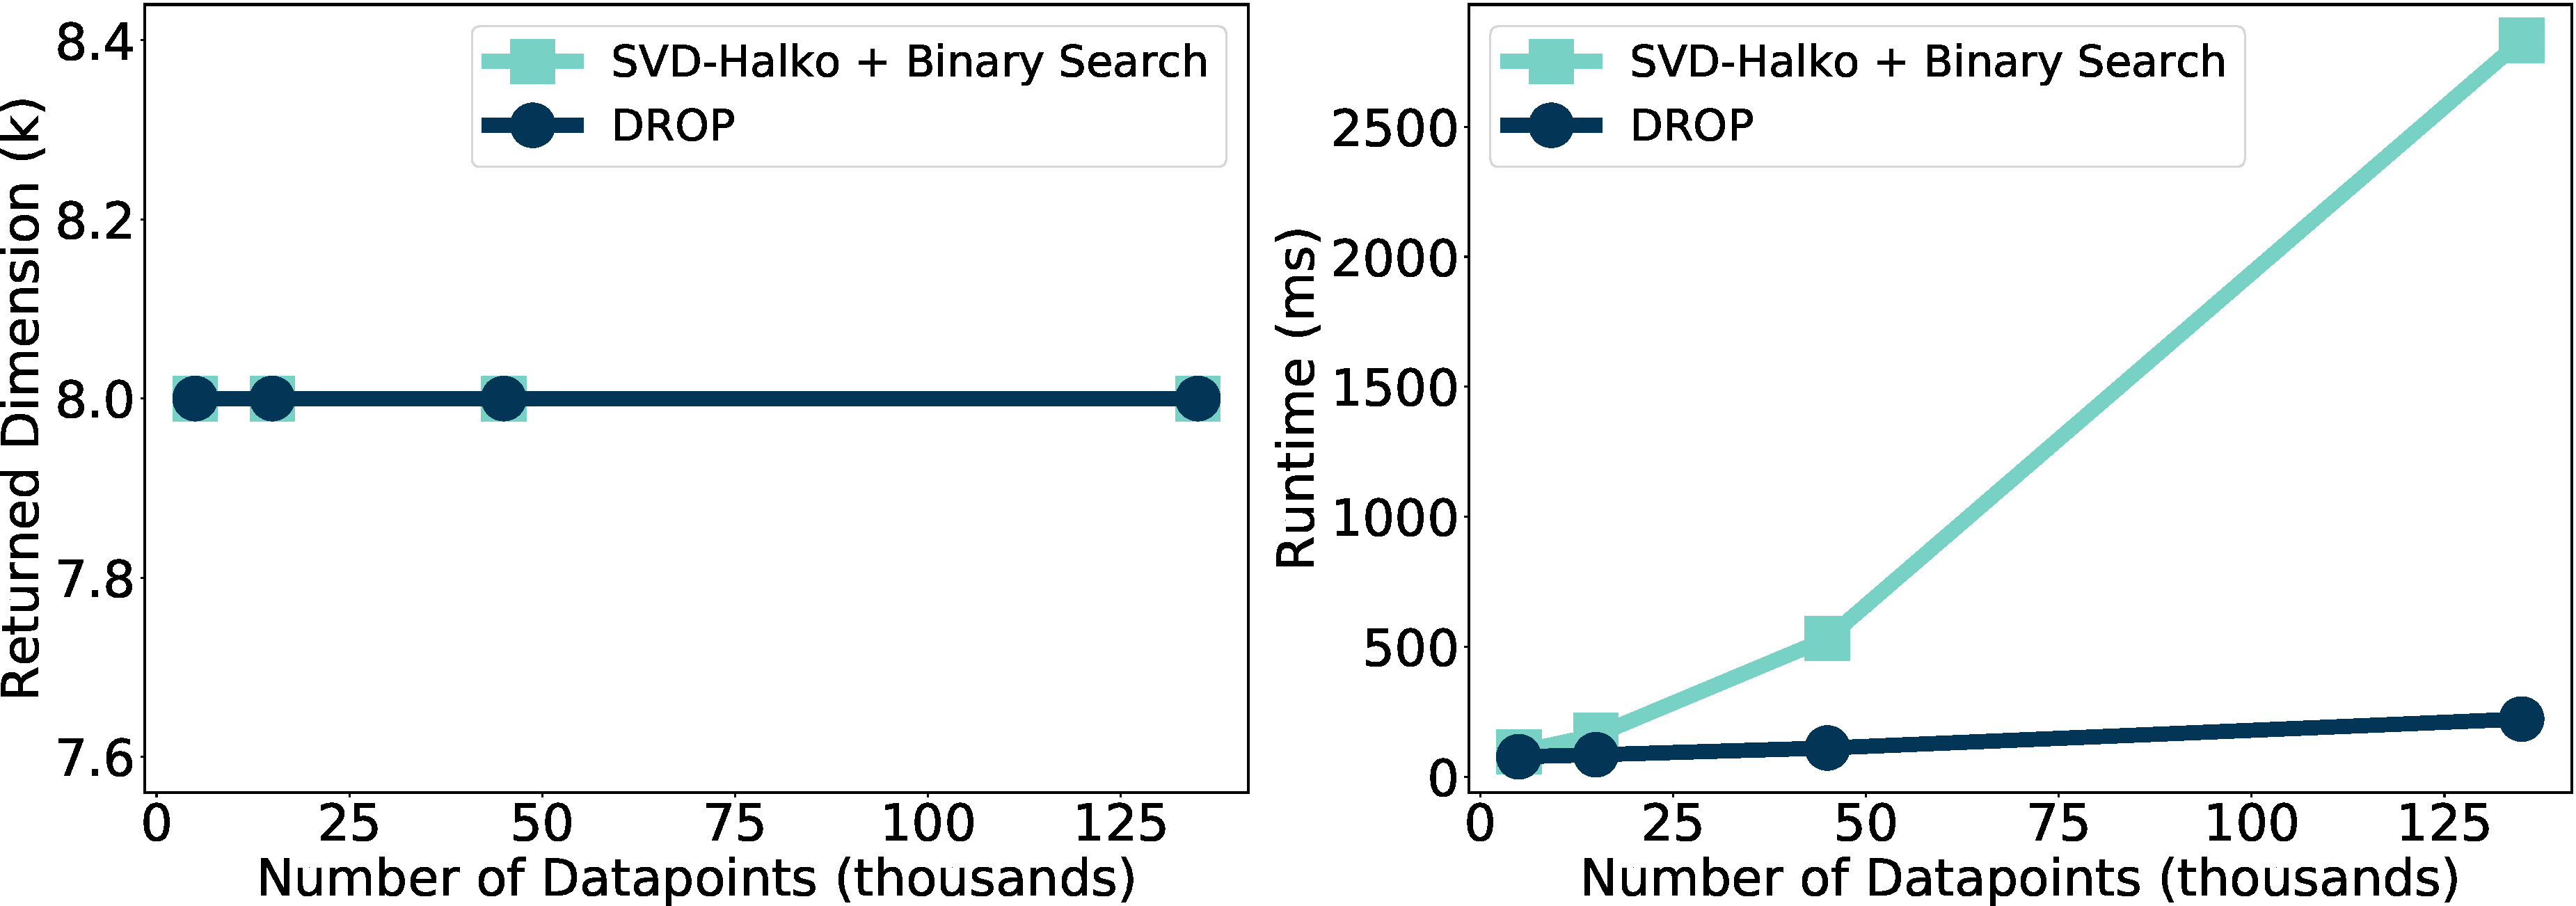
\includegraphics[width=\linewidth]{figs/increasing-revision.pdf}
\caption[]{Effect of dataset size on time and output dimension ($k$), with constant intrinsic data dimensionality of 8. DROP runtime with a fixed schedule remains near constant.}
\label{fig:increasingdata}
\end{figure}

\end{comment}


\begin{figure}
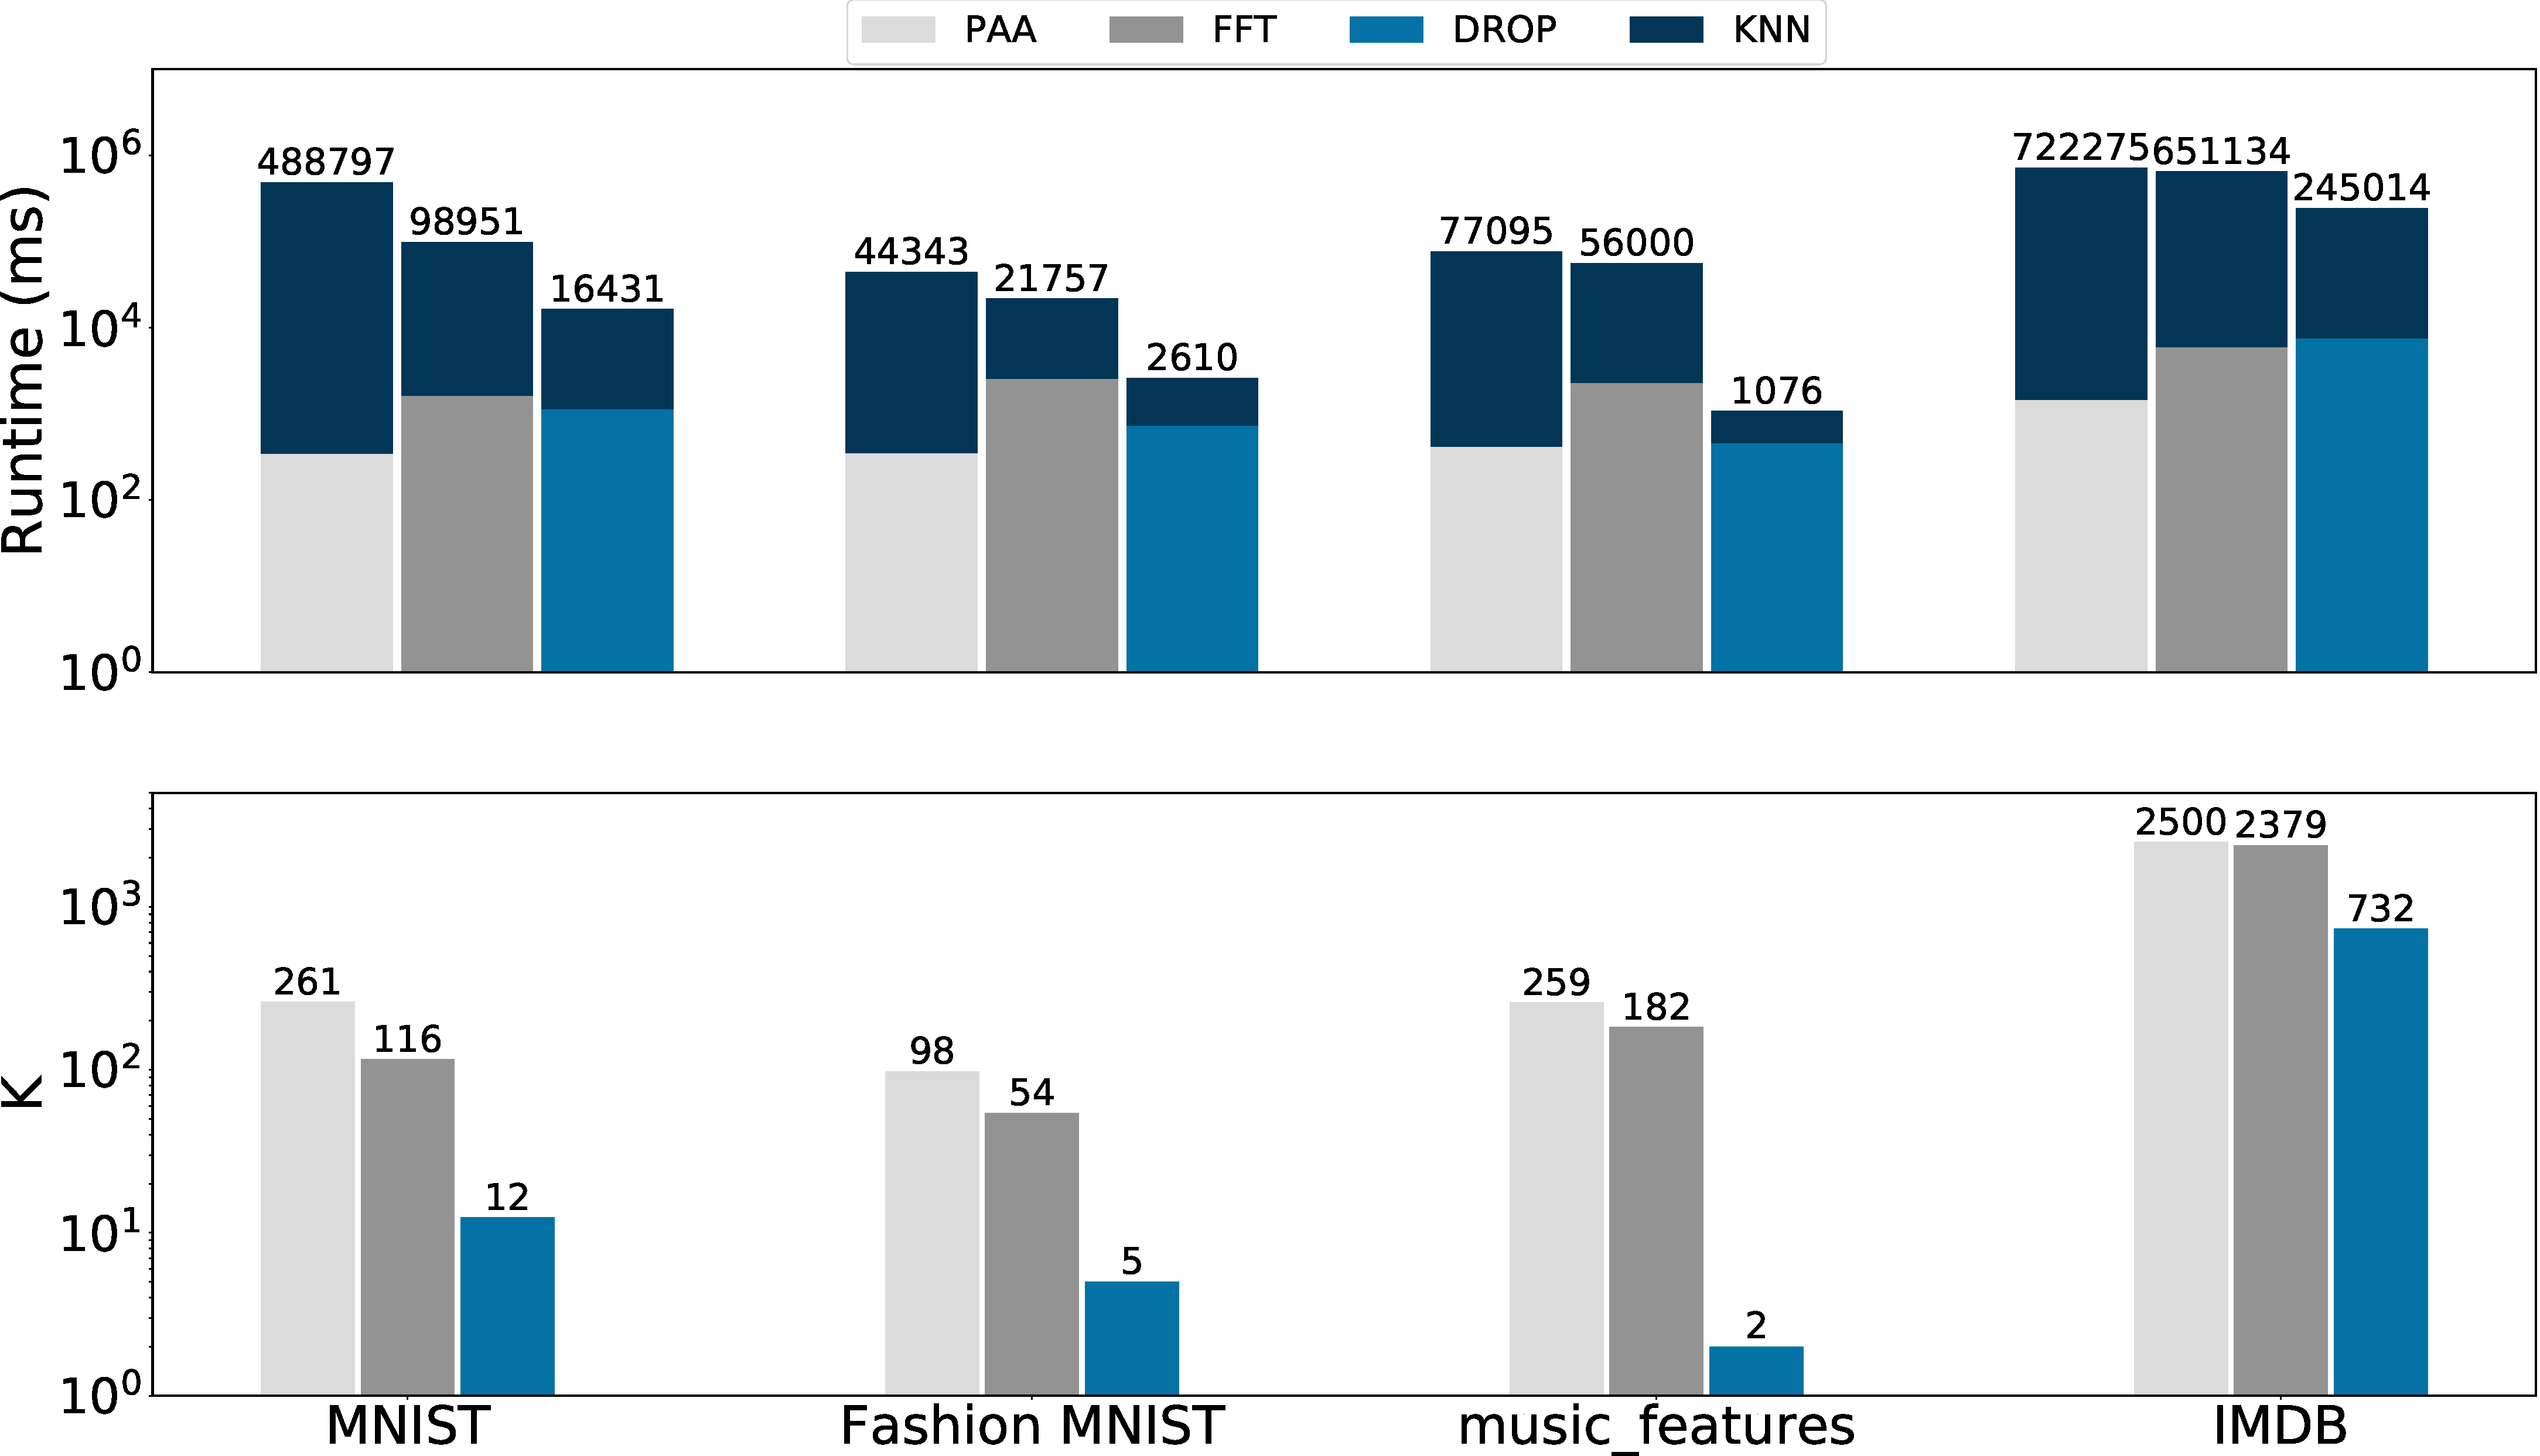
\includegraphics[width=\linewidth]{figs/nonts-revision.pdf}
\caption[]{End-to-End k-NN runtime (top) and returned dimension $k$ (bottom) over the entire MNIST dataset and the FMA featurized music dataset.}
\label{fig:beyond}
\end{figure}

\red{
\subsection{Beyond Time Series}
\label{subsec:nonts}

We consider generalizability beyond our initial case study along two axes: data domain and downstream workload. %These preliminary results show promise in extension to additional domains and target tasks.  

\subsubsection*{Data Domain}
We examine classification/similarity search workloads across image classification, music analysis, and natural language processing. 
}
We repeat the k-NN retrieval experiments with a 1:1 index-query ratio.
We use the MNIST hand-written digit image dataset of 70,000 images of dimension 784 (obtained by flattening each $28 \times 28$-dimensional image into a single vector~\cite{mnist}, combining both the training and testing datasets); FMA's featurized music dataset, providing 518 features across 106,574 music tracks; a bag-of-words representation of an IMDb sentiment analysis dataset across 25,000 movies with 5000 features~\cite{imdb}; \red{Fashion MNIST's 70,000 images of dimension 784~\cite{fashion}}.  
We present our results in Figure~\ref{fig:beyond}.
As these datasets are larger than those in~\cite{ucr}, DROP's ability to find a $TLB$-preserving low dimensional basis is more valuable as this more directly translates to significant reduction in end-to-end runtime---up to \red{a 7.6 minute wall-clock improvement in MNIST, 42 second improvement in Fashion MNIST, 1.2 minute improvement in music features, and 8 minute improvement in IMDB compared to PAA. 
These runtime effects will only be amplified as the index-query ratio decreases, to be more typical of the repeated-query setting. 
For instance, when we decrease the ratio to 1:5 on the music features dataset, DROP provides a 6.1 and 4.5 minute improvement compared to PAA and FFT, respectively. 
}

\red{
\subsubsection*{Downstream Workload}
To demonstrate the generalizability of  DROP's pipeline as well as black-box runtime cost-model estimation routines, we extend our pipeline to perform a k-means task over the MNIST digits dataset. 
We fit a downstream workload runtime model as we did with k-NN, and operate under a 1:1 index-query ratio. 
DROP terminates in 1488ms, which is 16.5$\times$ and 6.5$\times$ faster than PAA and FFT. 
}



\begin{comment}
\subsection{PCA Subroutine Evaluation}
\label{subsec:pcaexp}

PCA algorithms  are optimized for different purposes, with varying convergence, runtime, and communication complexity guarantees. 
DROP is agnostic to choice of PCA subroutine, and improvements to said routine provide complementary runtime benefits. 
\red{To implement DROP's default algorithm, we use MTJ and netlib-java linked against Intel MKL. 
Our SVD subroutine is competitive with the commonly used SciPy library~\cite{scipy} in Python linked against Intel MKL. 
We provide a plot of the runtimes over the UCR datasets (original, and number of datapoints inflated by $5\times$).

We also provide implementations of PCA via SMILE, Probabilistic PCA via SMILE's implementation, and PCA via (stochastic) Oja's method (not linked against Intel MKL) as a proof-of-concept of DROP's modularity, but they perform orders of magnitude slower than the optimized default.}



\begin{figure}
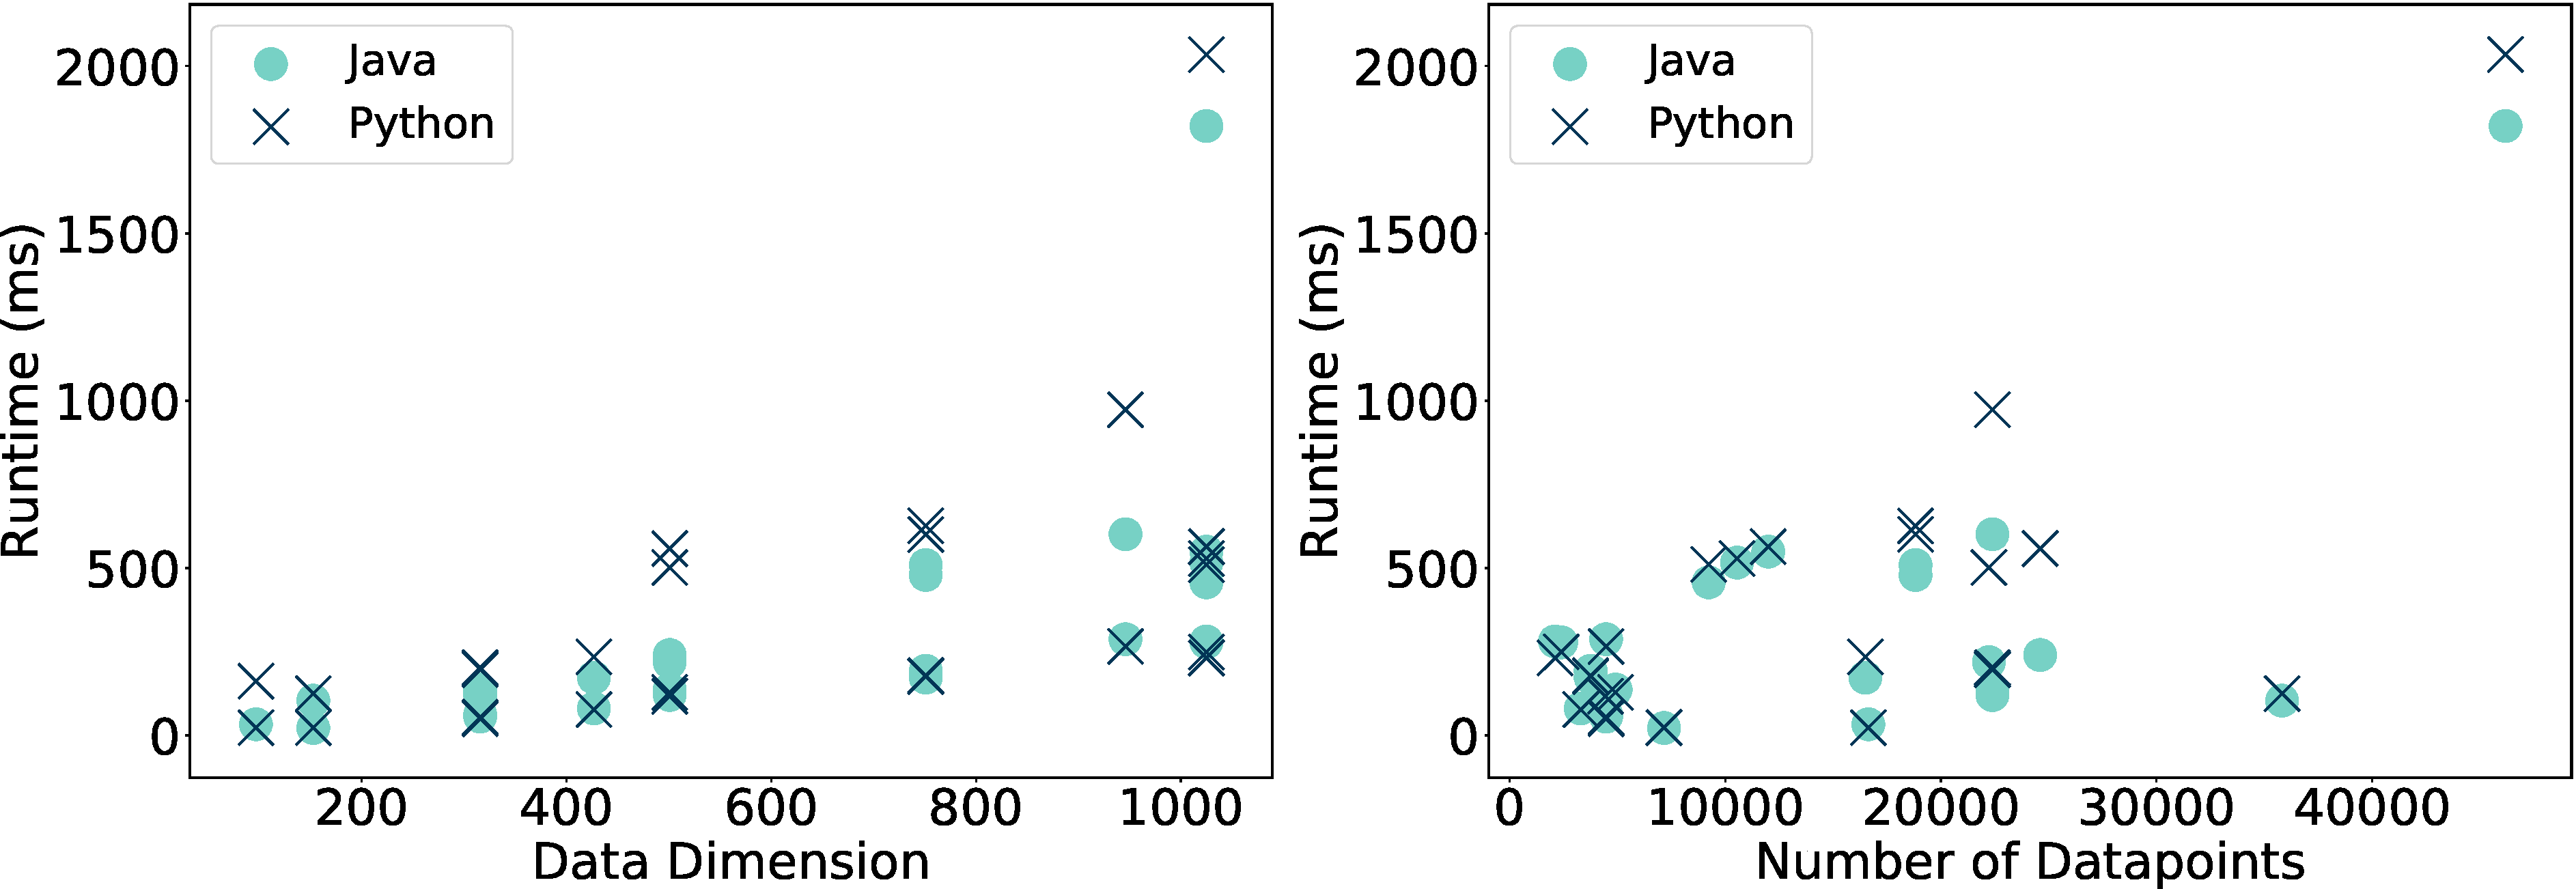
\includegraphics[width=\linewidth]{figs/runtime-revision.pdf}
\caption[]{Comparison of DROP's java PCA implementation with Python (SciPy) over the UCR datasets. }
\label{fig:pca_comp}
\end{figure}
\end{comment}






     

 
